\documentclass[./thesis.tex]{subfiles}

 
\begin{document}

\section{def}

\section{PT2 vs CIPSI}

CIPSI and PT2 both involves computing all $\epsilon(\alpha)$, so both can be computed at the same time. However, there are two problems.
\begin{itemize}

\item
At iteration $n$, CIPSI builds $\Psi_n$ while PT2 estimates the cost of trunction for $\Psi_{n-1}$. Computing PT2 for a "final" wavefunction $\Psi_n$ therefore requiers an extra iteration, which applies to a larger $\Psi$. ( autres implementation de PT2 possible ).

\item
As was said in SELECTION, the CIPSI algorithm can take pretty drastic approximations. We can only explore a small subset of $\ket \alpha$ in which we are almost sure to find all those with the greatest contribution $\epsilon(\alpha)$ ( $t_g$ threshold ), and do not need a very accuate value for that contribution as we are only trying to identify the large ones ( $t_s$ threshold ). However, it is not the same when computing the PT2. The very large number of smaller contributions makes them much harder to neglect. Unfortunately, increasing $t_g$ and $t_s$ thresholds dramatically increases the computational cost.

\end{itemize}

Given those, the best choice was to set low thresholds for $t_g$ and $t_s$ while performing CIPSI and accept the grossly truncated values for PT2, and highen them just for the last iteration, resulting in a very costly PT2 computation. In fact setting $t_g = t_s = N_{det}$ usually resulted in prohibitively long computation, so the final PT2 was still truncated.

\section{Stochastic PT2}
This issue was eventually solved by turning our deterministic PT2 computation into a stochastic one.

\paragraph{Initial note : ``Sample'' and ``Comb''}
Because of its original nature, this algorithm casts some ambiguity on what should be refered to as a ``sample''. We are going to estimate a sum of elementary contributions $E(I)$, compute and store them individually, and draw them based on a repartition function ; therefore they will be refered to as the \emph{samples}. But the values actually treated as samples in the statistical sense, are sums over several $E(I)$, refered to as \emph{combs}.



\paragraph{}  Since $\epsilon	(\alpha)$ is an energy contribution it's necessarily negative, PT2 is a sum of same-sign contributions. Therefore, truncating it inevitably results in a bias, it's known some energy is missing, but there is little clue how much exactly. The $t_g$ and $t_s$ thresholds used in CIPSI are ways of minimizing this truncation's amplitude for a given computational cost.
A better alternative, however, is to turn this bias into an error bar. Instead of trying to get the largest possible chunk of contribution, we can randomly pick $\epsilon(\alpha)$ contributions and make a Monte-Carlo estimate for the sum over all $\ket \alpha$. Not only the estimate will be much closer to the actual PT2, but we can have an estimation for the error. In this case, to avoid any bias
$$t_g = N_{gen} ; t_s = N_{det}$$

For different reasons, the actual Monte-Carlo computation is significantly more convoluted than simply drawing random $\ket \alpha$.

\paragraph{Individual $\epsilon(\alpha)$ are expensive to compute}
In the CIPSI algorithm, each generator determinant creates a number of unique $\alpha$, and computes $\epsilon(\alpha)$ for each one of them.
Essentially, $\ket \alpha$ are grouped in $N_{gen}$ disjoint batches, each associated with a generator determinant, as shown in figure \ref{fig:mu_sample}.

	$$\epsilon(\alpha) \in \mathcal{A}_i ; \Hij{\alpha}{\Psi_i} \neq 0 ; \Hij{\alpha}{\Psi_{j<i}} =0 $$

Because of the numerous tricks used, computing all $\epsilon(\alpha)$ from a batch at the same time is considerably faster than computing each separately. Therefore, in order to access a larger chunk of data, the stochastic PT2 algorithm will not consider individual $\epsilon(\alpha)$, but instead sums of all $\epsilon(\alpha)$ from the same batch.
The elementary contributions we are considering, aren't $\epsilon(\alpha)$, but
	$$E(I) = \sum_{\alpha \in \mathcal{A}_I} \epsilon(\alpha)$$
Indeed
    $$E_{PT2} = \sum_{I} E(I)$$
    
$E(I)$ are already explicitely computed by our CIPSI implementation, which returned the aggregated values of $\epsilon(\alpha)$ for one job, one job being essentially a generator.

\paragraph{There are few elementary contributions}
Each elementary contribution is associated with a generator determiant. There are only $N_{gen}$ elementary contributions. This is small enough so, when a $E(I)$ contribution is computed, its value can be stored and simply re-used if the same sample is drawn again. This, in turn, means the exact result will eventually be known once every sample has been computed. The cost for this will essentially be the same as that of the purely deterministic computation, with a negligible additional cost due to the Monte-Carlo related computations ( drawing random numbers, finding the associated samples... ).

\paragraph{The elementary contributions are decreasing with $I$}
	Variational determinants are sorted in decreasing absolute values of $C_I$.
	The values of $E(I)$ span many orders of magnitude and decrease rapidly with $I$, in an exponential-ish way. Smoothed values for $E(I)$ are shown in figure \ref{fig:p_i}. There are a few reasons for that.
\begin{itemize}
	\item
	The values for $\Delta E_\alpha$ used in the computation of $\epsilon(\alpha)$ tend to increase, as variational determinants tend to be more and more excited and to populate higher orbitals ( detailler ? )
	\item
	The number of unique $\ket \alpha$ per generator decreases. Indeed, the more ``previous generators'' there is, the likelier it is that a generated $\ket \alpha$ was generated before.
	\item
	Unique $\ket \alpha$ are, by construction, disconnected from all previous generators, which mean they connect to a smaller and smaller norm of $\Psi$ ( see figure \ref{fig:a_con} ). 
\end{itemize}
It is not ideal for a Monte-Carlo computation to deal with sample values that span many orders of magnitude. A repartition function can alleviate the issue to some extent.
The last reason given for the decrease of $E(I)$ is the most important one, and leads us to consider
$$\tilde w_i = C_i^2$$
as a repartition function for $E(I)$ (detailler un poil). This is however not the exact repartition function used in the Monte-Carlo scheme. We will later introduce some slight modifications to it, for algorithmic reasons. As can be seen in figure \ref{fig:eici2}, $$p_I = \frac{E(I)}{C_I^2}$$ is  still similar to $E(I)$ in that it span orders of magnitudes and decreases rapidly.
This can be taken advantage of in two ways
\begin{itemize}
\item
Values in a small range of $p_I$ are relatively close. The entire space of $p_I$ is separated in $N_{teeth}$ ranges refered to as \emph{teeth}. In figure \ref{fig:p_i}, the space of $p_I$ has been split in four teeth $P_1$ to $P_4$. The variance inside each tooth is expected to be, quite clearly, much smaller than the variance for the whole space.

As a matter of fact, the values actually sampled, are sums of 1 sample taken in each subspace, so-called ``combs''.
Essentially, the sum of ``one large, one average and one small'' has a lower variance than the sum of ``three at random''.
\item
Most of the contribution is contained in the first samples. We can entierely compute the first samples, and only make a stochastic estimation for the sum of the smaller ones. This effectively splits $E(I)$ in two ranges, a deterministic one, then a stochastic one (hence the hybrid characteristic of this method), and our estimated energy

$E = E_D + E_S$

with $E_D$ the exact energy for the deterministic part, and $E_S$ the estimated energy of the stochastic part. The error bar only applies to $E_S$, which is a fraction of the whole sum.
We have to define the threshold between those two ranges. A simple solution would be to arbirarily define it based on $c_I$.
But because we have already defined ranges as teeth, we take a dynamical, more flexible approach : given the first $E(I)$ that has not been computed yet by the Monte-Carlo scheme, and $P$ the tooth it belongs to, the deterministic range extends to $P$, exclusive.
\end{itemize}

So far, not all details have been dealt with, but this already makes if for a somewhat convoluted drawing scheme.

We are sampling combs, but we have defined a repartition function for $E(I)$. What does this mean? Since we impose that the same number of $E(I)$ are drawn in each tooth - one per comb - we effectively give all teeth the same weight $N_{teeth}^{-1}$ in the Monte-Carlo scheme. Therefore, the actual weight given to $E(I) \in P_x$ is

$$w_I = \frac{\tilde w_I}{N_{teeth} \times \sum_{J \in P_x} \tilde w_J}$$

To leave the repartition function unaltered, we need all teeth to actually weight $N_{teeth}^{-1}$, in other words

$$\sum_{J \in P_x} \tilde w_J = N_{teeth}^{-1}$$

Clearly this is not acheivable for any reartition function $\tilde w$. Schematically, it would require the threshold between two teeth to exactly match the threshold between two $E(I)$. It is possible to artificially split a $E(I)$ to get a matching threshold, but this adds some complexity algorithmically speaking.



For reasons that will be explicited later, all teeth are supposed to contain at least ~10 samples. Therefore, a simpler solution is to ``round'' the teeth thresholds to the $E(I)$ threshold directly above, which will result in teeth with a weight close to $N_{teeth}^{-1}$, and thus the actual repartition function will be little different from the one we initially defined. Since our repartition function is an extremely rough estimation of $E(I)$, to say the least, it is unlikely to cause any significant change in convergence speed.
Essentially, we will use $\tilde w$ only to define teeth, then use $w$ as the actual repartition function. This gives us, by definition, teeth weighting exactly $N_{teeth}^{-1}$.


SCHEMA




\begin{figure}[h!]
	\begin{center}
		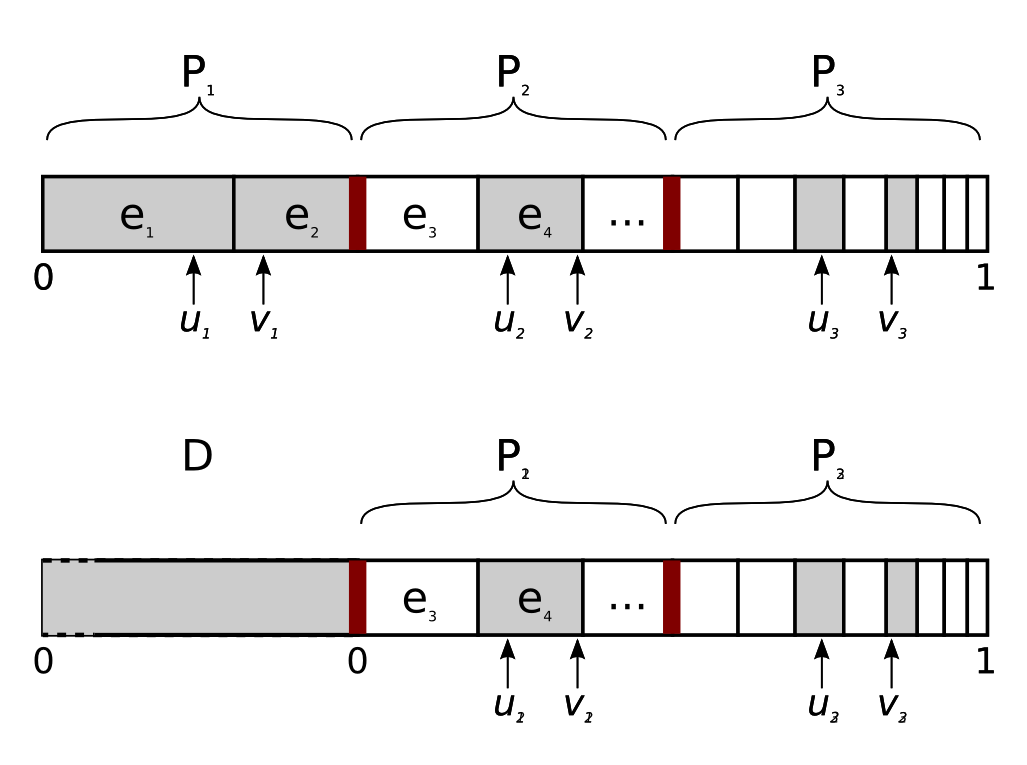
\includegraphics[width=0.9\columnwidth]{figures/pt2/move_to_deterministic}
		\caption{A REFAIRE NOTATION.............}
		\label{fig:move_to_deterministic}
		$E(I)$
	\end{center}
\end{figure}


\begin{figure}[h!]
	\begin{center}
		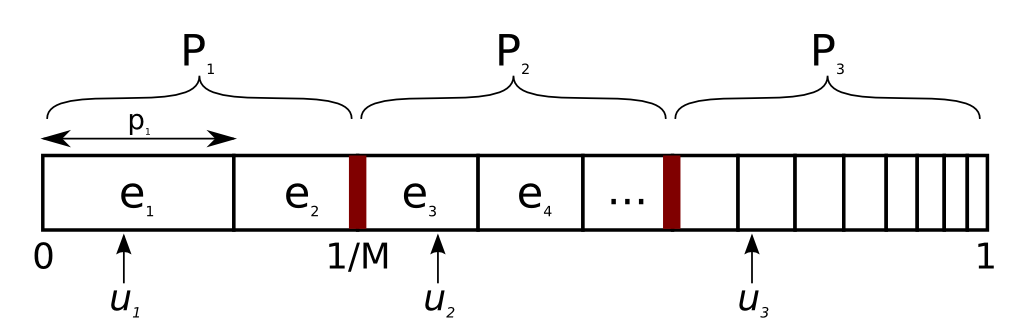
\includegraphics[width=0.9\columnwidth]{figures/pt2/comb}
		\caption{A REFAIRE NOTATION.............}
		\label{fig:comb}
		$E(I)$
	\end{center}
\end{figure}


\begin{figure}[h!]
	\begin{center}
		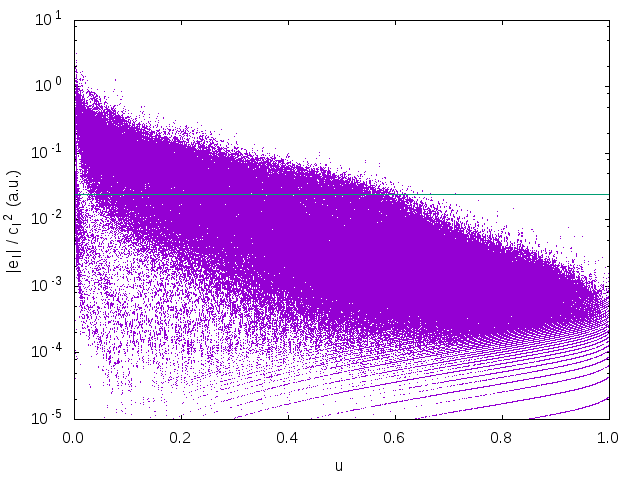
\includegraphics[width=0.9\columnwidth]{figures/pt2/eici2}
		\caption{A REFAIRE NOTATION.............}
		\label{fig:eici2}
		$E(I)$
	\end{center}
\end{figure}


\begin{figure}[h!]
	\begin{center}
		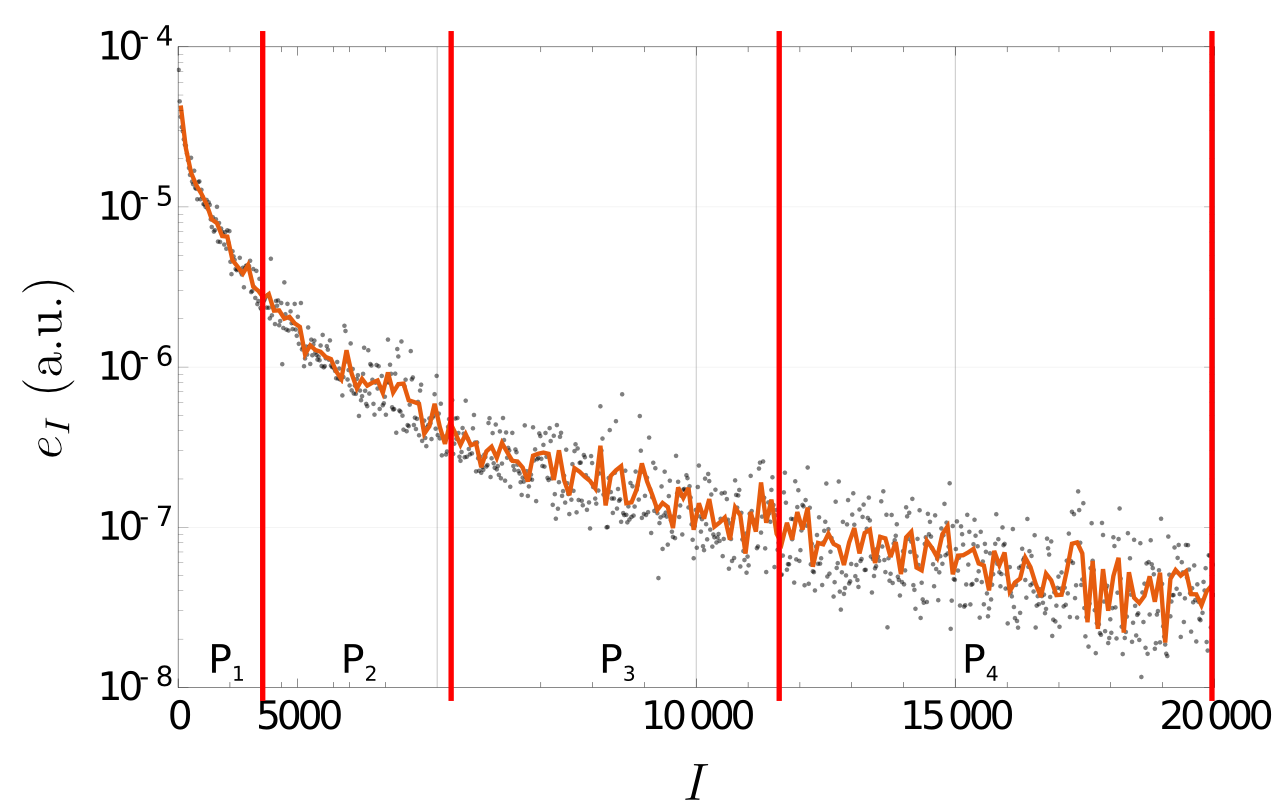
\includegraphics[width=0.9\columnwidth]{figures/pt2/P_i}
		\caption{A REFAIRE NOTATION.............}
		\label{fig:p_i}
		$E(I)$
	\end{center}
\end{figure}


\begin{figure}[h!]
	\begin{center}
		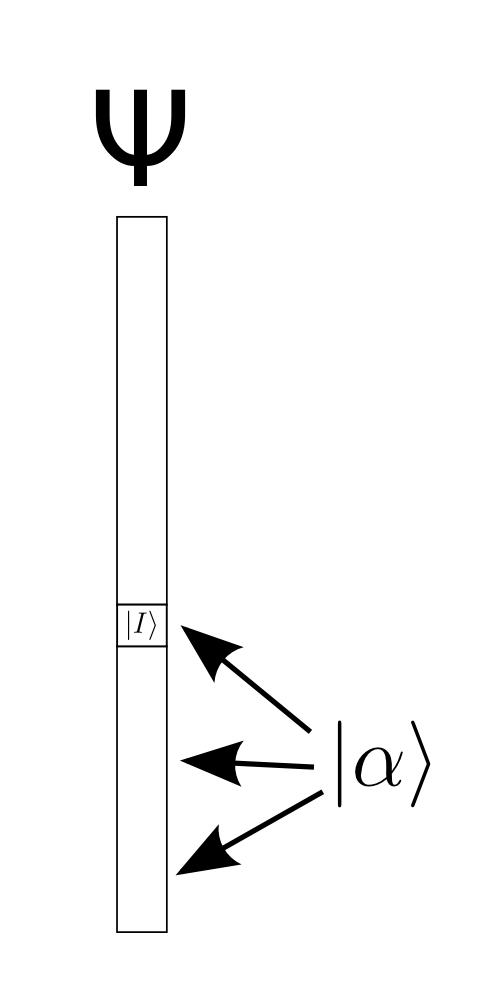
\includegraphics[width=0.2\columnwidth]{figures/pt2/a_con}
		\caption{A REFAIRE NOTATION.............}
		\label{fig:a_con}
		$\ket \alpha$ generated by increasing $\Psi_i$ connect to smaller and smaller norm of $\Psi$.
	\end{center}
\end{figure}

\begin{figure}[h!]
	\begin{center}
		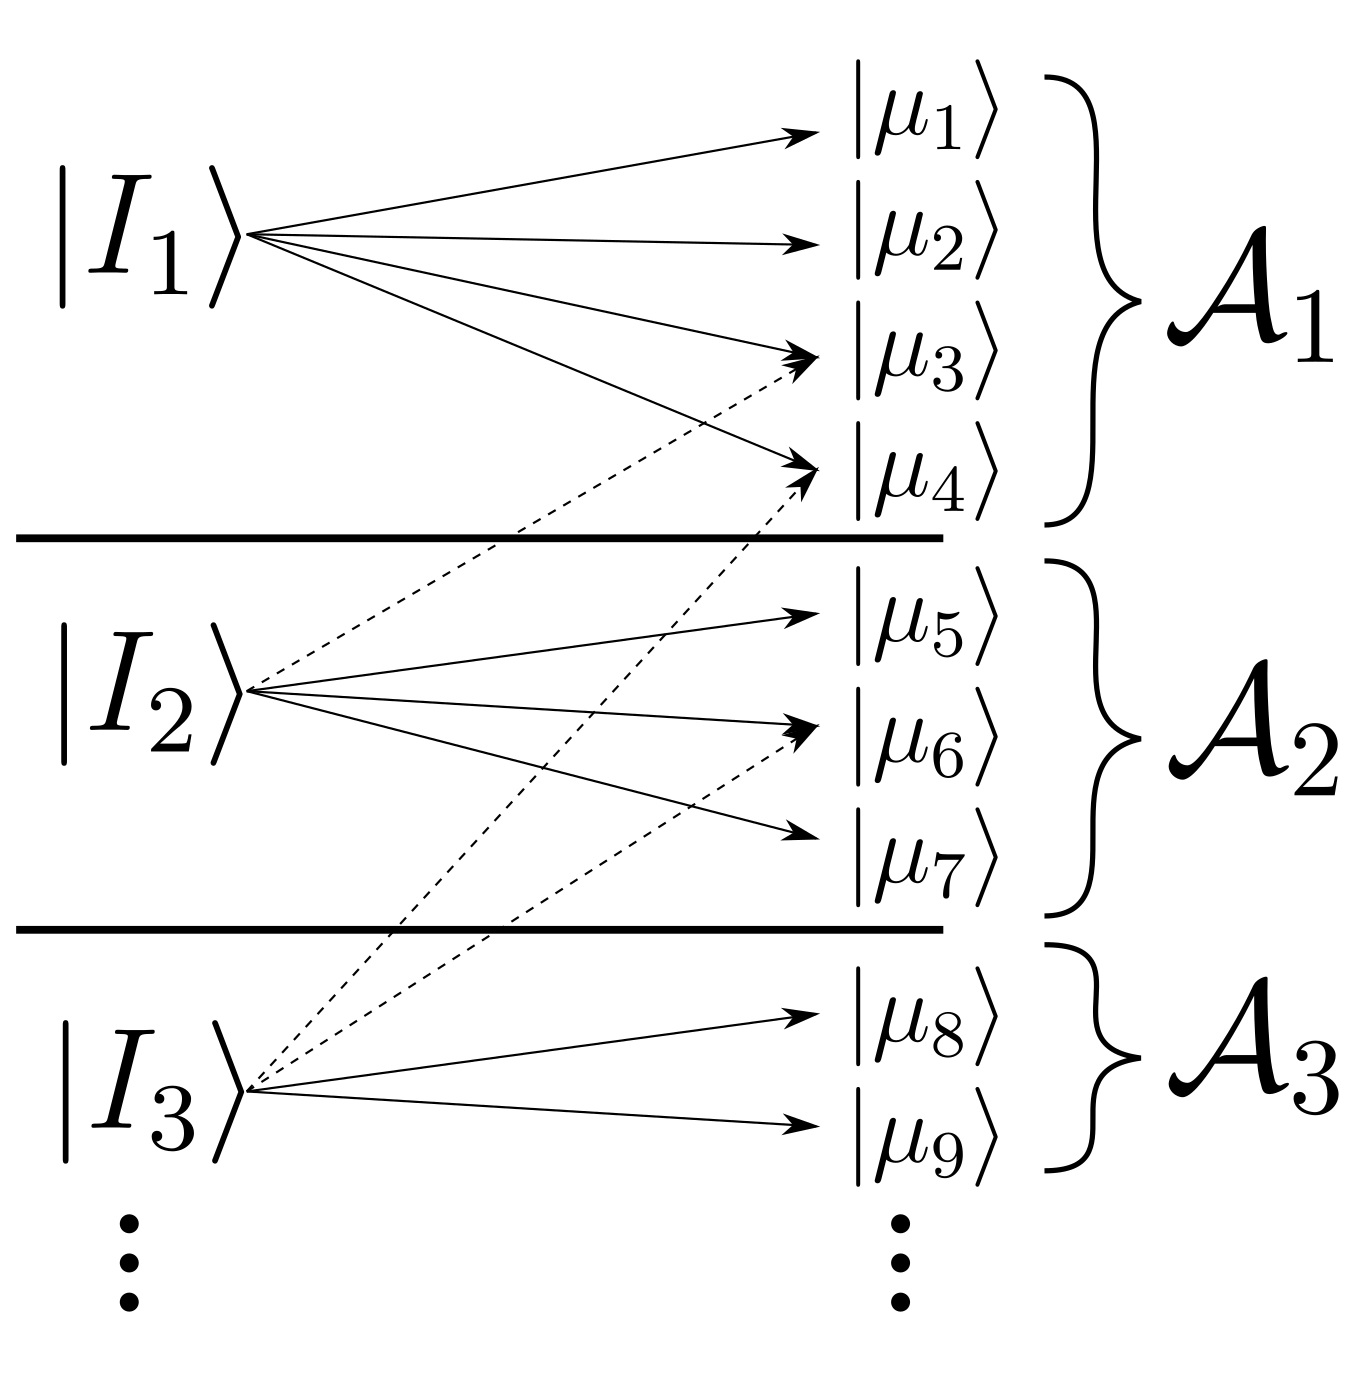
\includegraphics[width=0.5\columnwidth]{figures/pt2/mu_sample}
		\caption{}
		\label{fig:mu_sample}
		Construction of batches of $\ket \alpha$
	\end{center}
\end{figure}



\begin{figure}[h!]
	\label{comb_variables}
	\begin{center}
		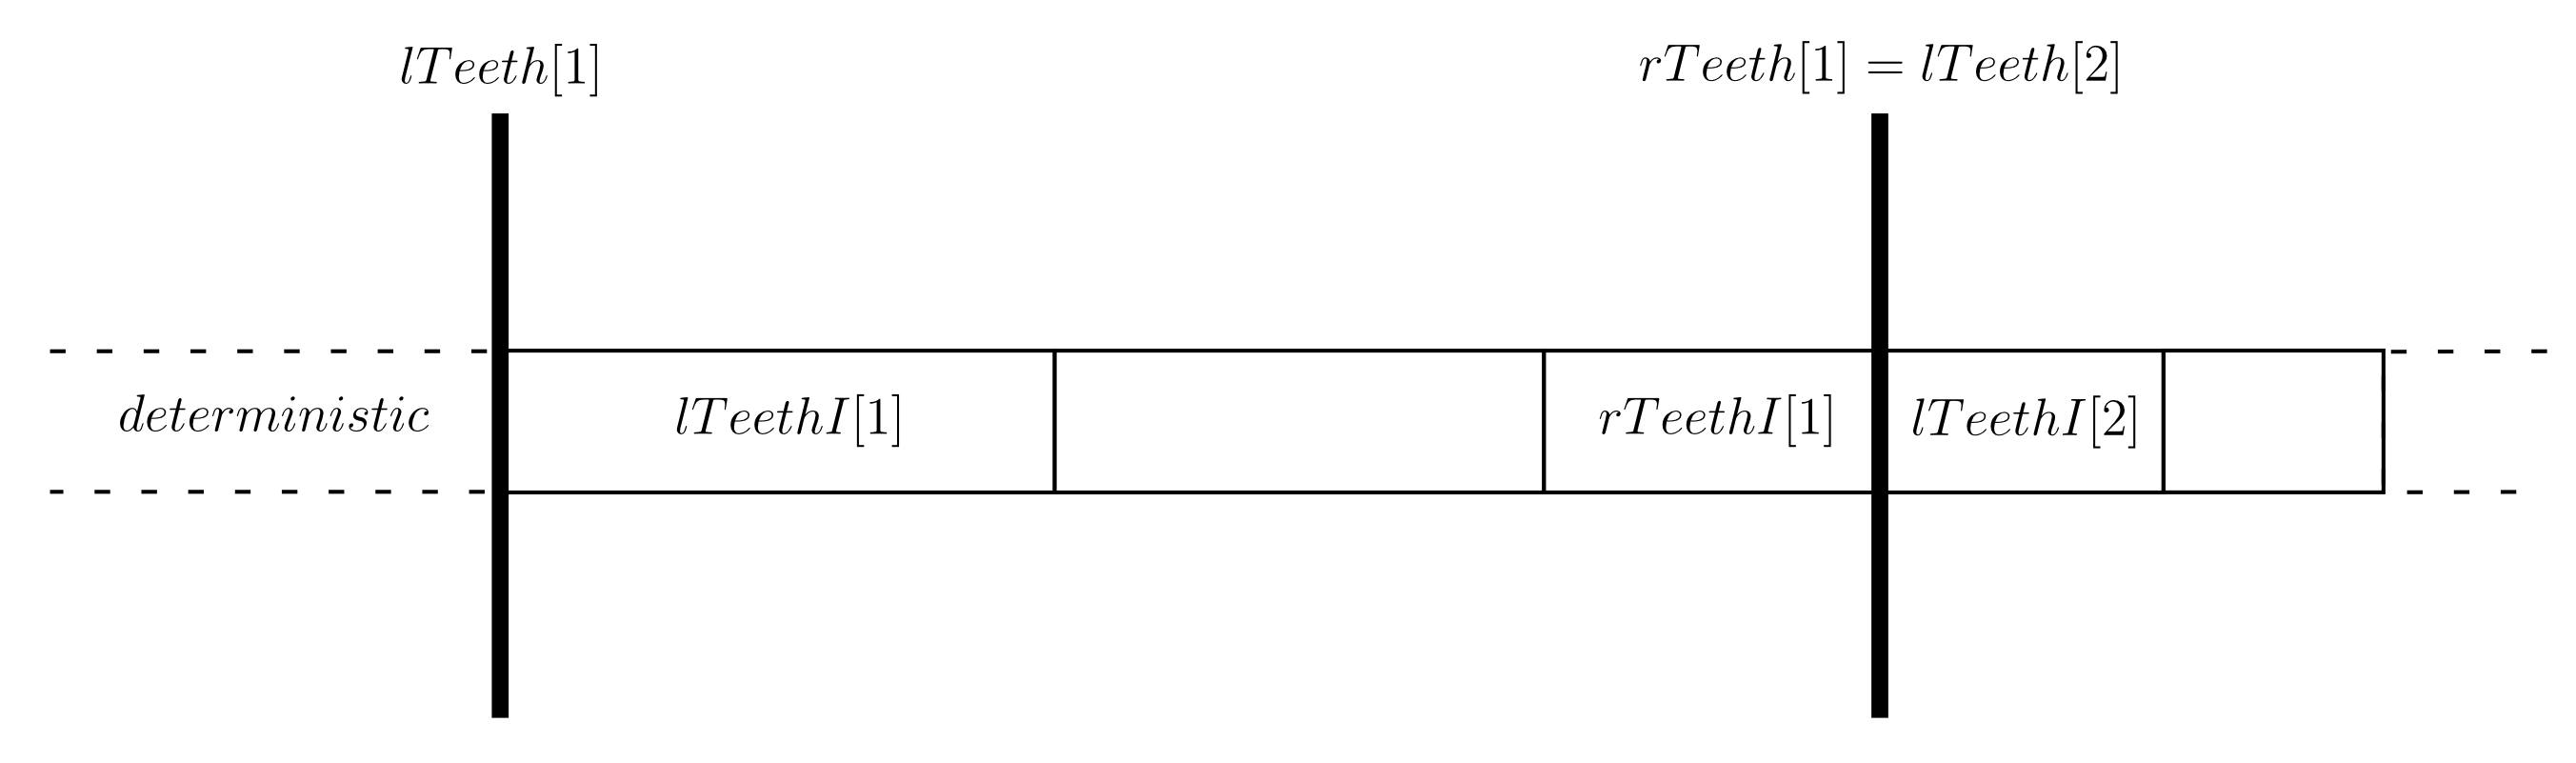
\includegraphics[width=1.00\columnwidth]{figures/pt2/teeth}
		\caption{comb}
		Variable names for the "comb" partition of $\Psi$. In boxes are shown indices, above are shown probabilities
		$$toothOfDet[i] = t ; i \in \big [ lTeethI[t],rTeethI[t] \big ]$$
		$$toothSize[t] = rTeeth[t] - lTeeth[t]$$
	\end{center}
\end{figure}

\begin{figure}[h!]
	\begin{center}
		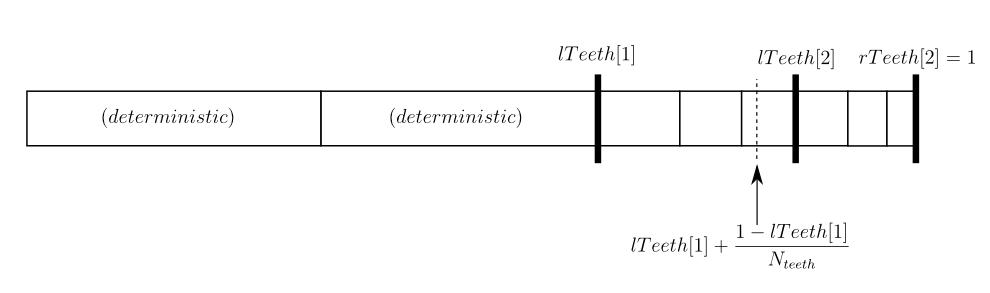
\includegraphics[width=1.00\columnwidth]{figures/pt2/teeths}
		\caption{\label{filtering}}
		Construction of teeth with $N_{teeth} = 2$ and 2 samples in the initial deterministic set.
	\end{center}
\end{figure}

\begin{figure}[h!]
	\begin{center}
		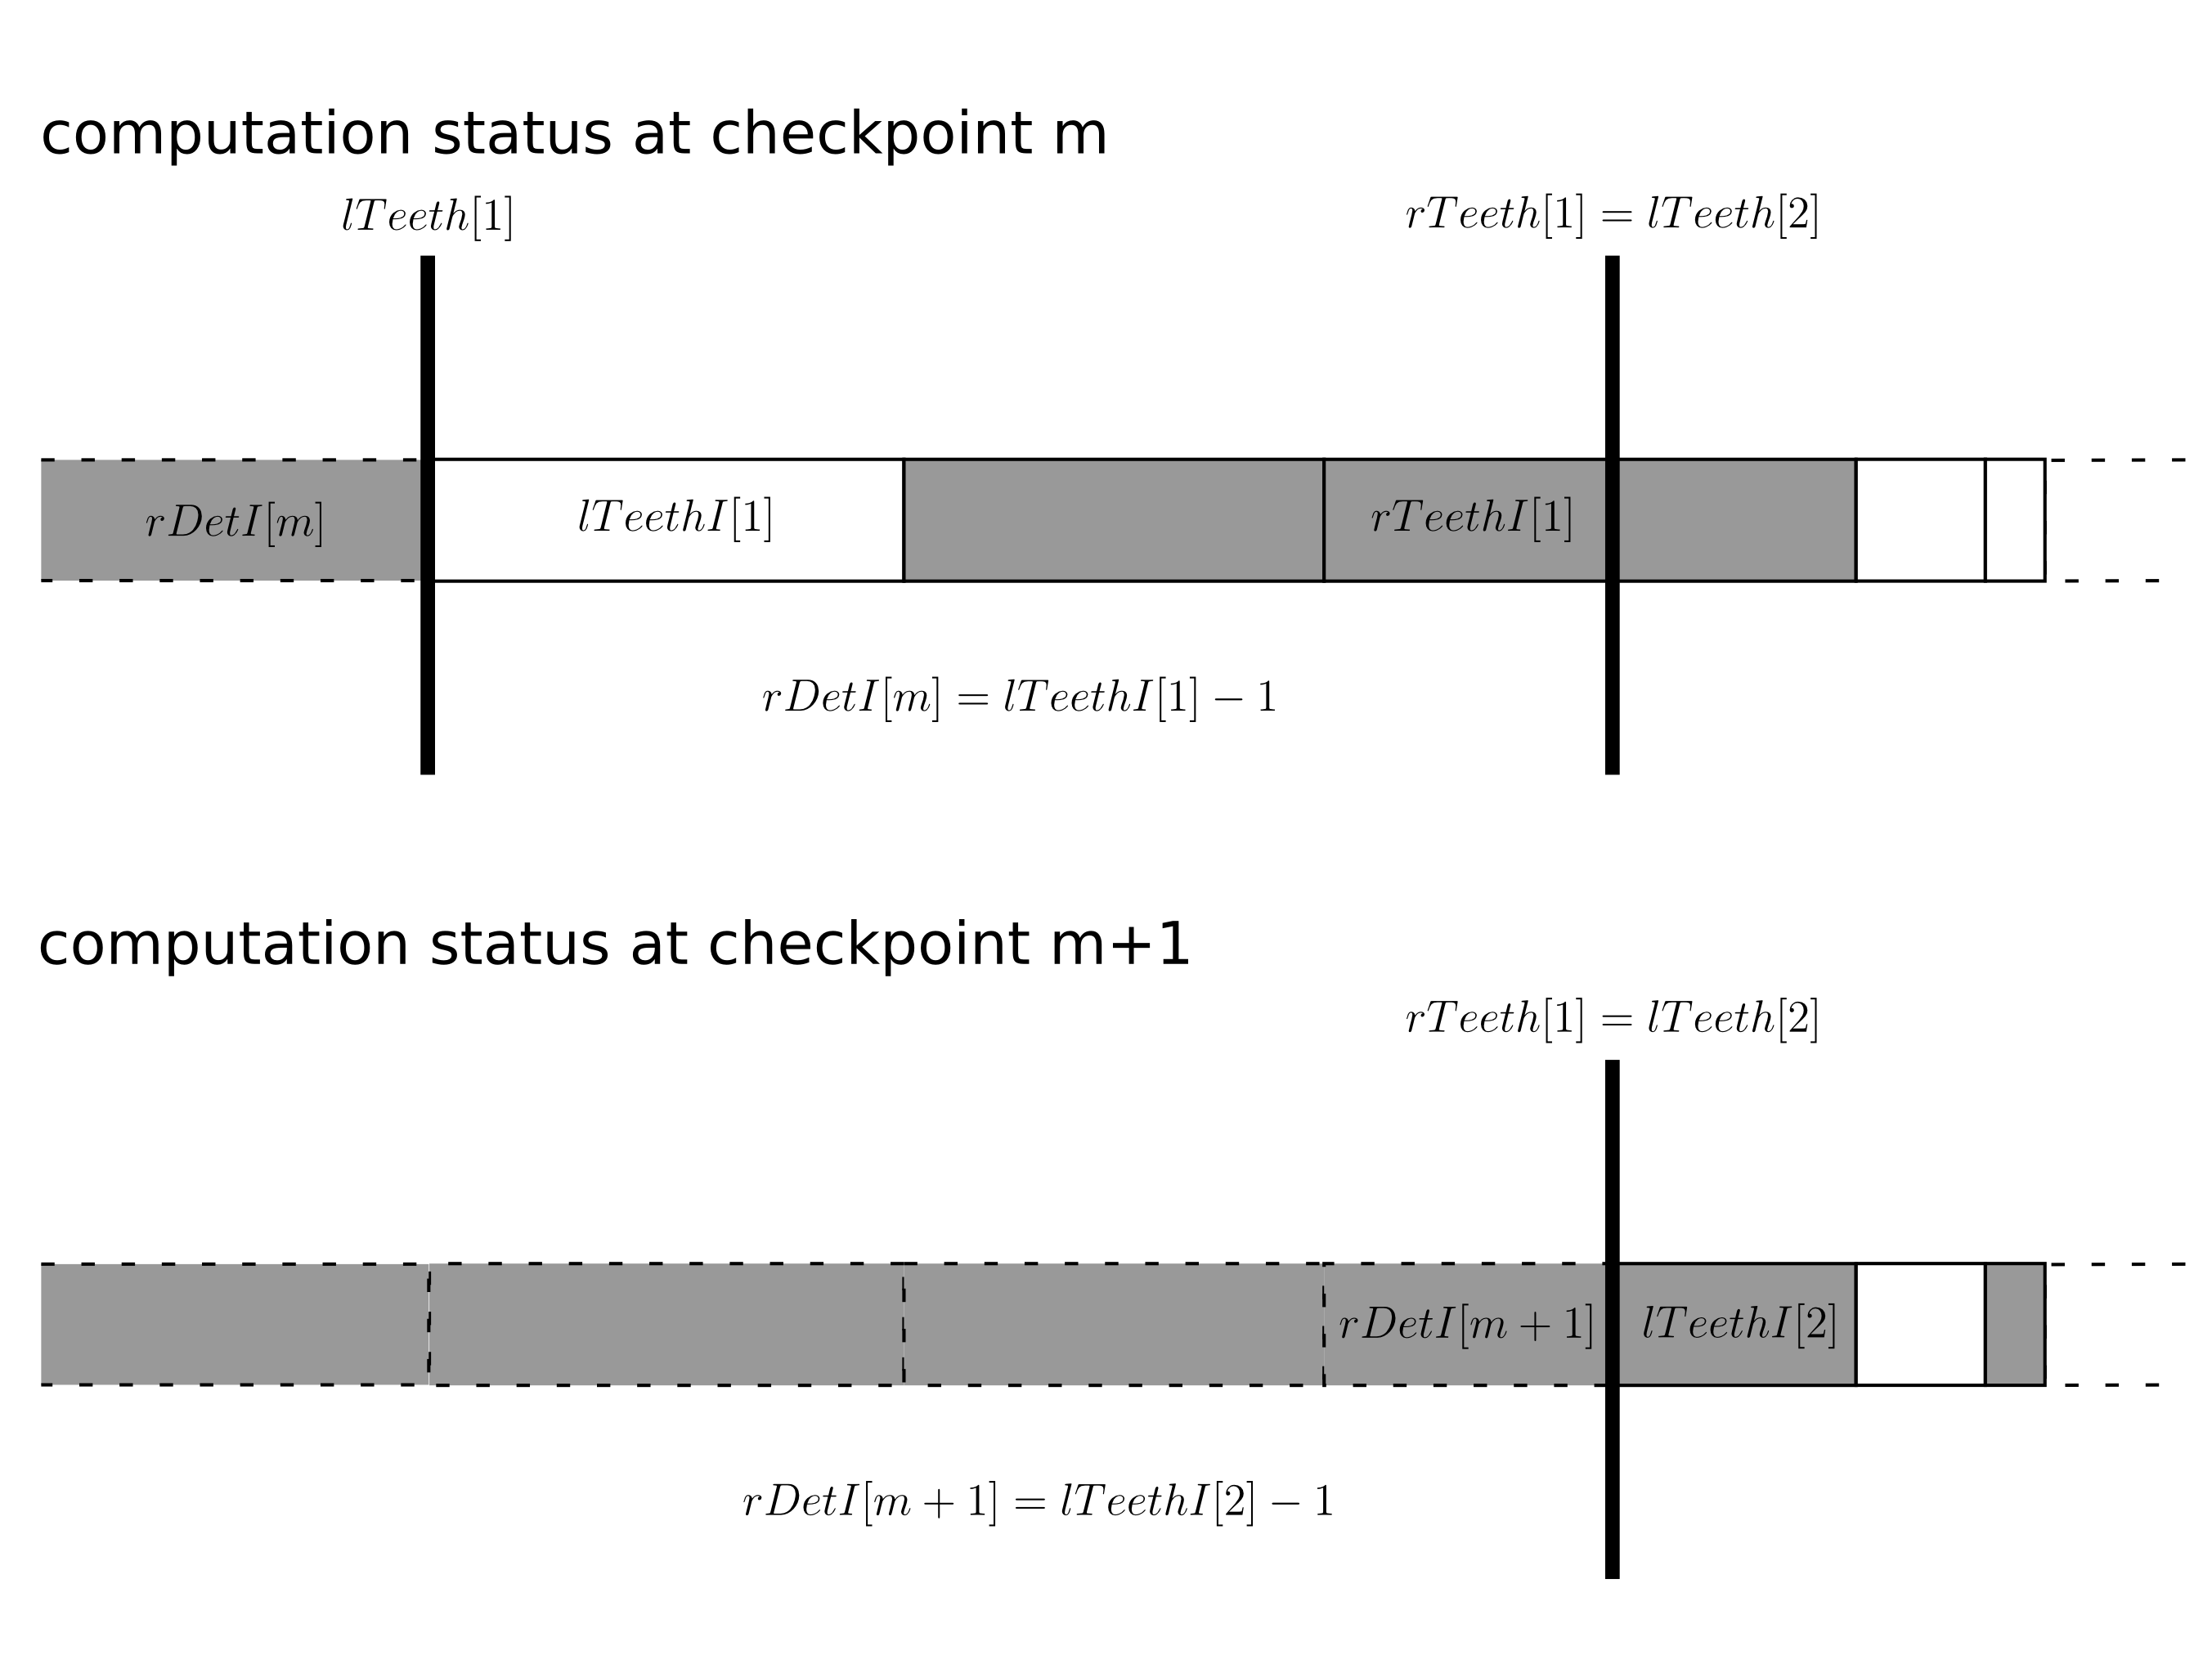
\includegraphics[width=1.00\columnwidth]{figures/matrix_dressing/deterministic_cp}
		\caption{\label{filtering}}
		$rDetI[m]$ gives the index of the last sample of the deterministic part at checkpoint $m$, or $0$ if there is no deterministic part.
		Greyed samples have been computed. Dotted samples are in the deterministic part. Sample $lTeethI[1]$ has been computed between checkpoints $m$ and $m+1$, resulting in tooth $1$ begin fully computed and thus moved into the deterministic part.
	\end{center}
\end{figure}

\end{document}
